Comme expliqué plusieurs fois précédemment, assurer la scalabilité de l'application est un point crucial de ce travail de Bachelor. En effet, l'application doit tenir la charge d'un nombre de festivaliers potentiellement important en simultané.

\section{Tests de montée en charge}

Afin de simuler un nombre important de festivaliers, il est nécessaire de mettre en place un outil permettant de simuler de réels utilisateurs. Dans la plupart des cas, ce type de test se contente de réaliser un nombre conséquent de requêtes HTTP sur l'application afin de vérifier diverses métriques. Dans le cas de \gls{beeplace}, il ne s'agirait pas d'une solution très intéressante. En effet, l'obstacle majeur à la scalabilité de l'application est la communication WebSocket, qui s'occupe de toute la synchronisation des données entres les utilisateurs. En effet, aucun appel HTTP n'est réalisé par le client vers le serveur, toute l'information transite par WebSocket. Aussi bien l'état initial du canvas que la pose d'un pixel ou encore la réception des pixels des autres utilisateurs. Il faut donc avoir cet aspect bien à l'esprit lors du choix de l'outil de test.

\subsection{Déploiement de l'application}

Afin de tester les limites de l'application sans affecter la version en production, l'application est déployée sur une seconde machine virtuelle à l'adresse suivante \href{https://dev-place.beescreens.ch}{dev-place.beescreens.ch}. Les spécifications de cette machine virtuelle sont les suivantes:

\begin{itemize}
  \item CPU 4 c\oe{}urs Intel(R) Xeon(R) CPU E5-2697 v4 @ 2.30GHz
  \item 4 Go de RAM
  \item 50 Go de disque
\end{itemize}

\gls{beeplace} est déployé sur cette machine virtuelle à l'aide de Docker et de Docker Compose. La configuration utilisée est la même que pour la version en production. Celle-ci est disponible dans le répertoire \mintinline[breaklines]{bash}{deployement/beeplace} du répertoire git.

\subsection{Choix de l'outil}

Pour pouvoir tester la communication WebSocket, il faut tester l'implémentation choisie, à savoir Socket.IO. En effet, Socket.IO utilise son propre protocole de communication~\cite{socket-io-protocol} au-dessus des WebSockets classiques, qui n'est pas forcément supporté par tous les outils de test. La documentation officielle de Socket.IO propose deux manières~\cite{socket-io-load-testing} de tester une application utilisant Socket.IO:

\begin{enumerate}
  \item Utiliser l'outil Artillery~\cite{artillery}
  \item Créer un nombre important de clients Socket.IO manuellement
\end{enumerate}

La deuxième solution n'est pas l'idéale car elle ne permet pas d'avoir des statistiques très poussées sur les performances de l'application. En effet, il est compliqué de récupérer un nombre suffisant de métriques sans finir par développer son propre outil de test. Afin de ne pas réinventer la roue, le choix initial s'est porté sur Artillery.

\subsubsection{Artillery}

Artillery propose différents moteurs utilisables pour tester une application. Il existe donc un moteur Socket.IO permettant d'avoir une solution clé en main pour tester facilement \gls{beeplace}. Les tests sont définis dans un fichier de configuration YAML, qui permet de définir les différentes phases de test ainsi que le comportement des utilisateurs virtuels (appelés scénarios). Ce fichier YAML peut importer un fichier JavaScript afin d'ajouter de la logique supplémentaire aux tests.

\begin{listing}[h]
  \inputminted{yaml}{assets/figures/artillery-test.yml}
  \caption{Test de montée en charge avec Artillery}
  \label{listing:artillery}
\end{listing}

Le test d'exemple \ref{listing:artillery} génère 1000 utilisateurs en une minute (soit environ 16 à 17 utilisateurs par seconde). Chaque utilisateur va dessiner 3 pixels aléatoirement sur le canvas et attendre ensuite 30 secondes. Cette attente est importante car le client va recevoir les pixels des autres utilisateurs pendant cette période, ce qui simule un comportement plus réaliste. La logique pour générer un pixel aléatoire ainsi que la fingerprint sont définis dans le fichier JavaScript importé \mintinline[breaklines]{bash}{functions.js}.

Cette solution très simple à mettre en place semble idéale. Cependant, un nombre important de problèmes est survenu:

\begin{itemize}
  \item Le script lance parfois une erreur \mintinline[breaklines]{bash}{Error: Callback was already called.} qui stope l'exécution du test. Plusieurs personnes semblent avoir le même problème sur \gls{github}~\cite{artillery-callback-issue} mais aucune solution n'a encore été trouvée. Utiliser un outil qui n'est pas stable n'est pas envisageable.
  \item Artillery ne permet pas de tester facilement la communication du serveur vers les clients. En effet, l'outil est plus adapté à la communication client-serveur. Ce qui est problématique afin de récupérer par exemple la configuration du canvas ou encore les pixels des autres utilisateurs.
  \item Artillery ne met pas à disposition des métriques très utiles dans ses résultats concernant les WebSockets ou Socket.IO. En effet, il n'est pas possible de récupérer la latence de la connexion WebSocket, qui est l'indicateur le plus important dans le cas de \gls{beeplace}. Artillery met à disposition une métrique \mintinline[breaklines]{bash}{socketio.response_time} qui pourrait être intéressante mais malheureusement celle-ci ne dépasse pas les 4 millisecondes, même lorsque l'application n'arrive plus à répondre, ce qui est très peu réaliste.
\end{itemize}

Ces raisons ont poussé à abandonner Artillery et à chercher une autre solution. Le code source des recherches effectuées avec Artillery n'est plus disponible dans le répertoire \gls{beescreens} mais reste accessible via un commit spécifique \footnote{Voir commit no. \href{https://gitlab.com/beescreens/beescreens/-/merge_requests/255/diffs?commit_id=98e5e73eae3f9ed77026245cc727aa42728cac3b}{98e5e73eae3f9ed77026245cc727aa42728cac3b}}.

\subsubsection{k6}

k6~\cite{k6} est un outil de test de performance open-source écrit en Go. Il fait partie des outils de test de montée en charge les plus populaires avec plus de 20'000 stars sur \gls{github} et est utilisé par de nombreuses entreprises comme Amazon, Microsoft ou encore \gls{gitlab}. Son avantage principal dans le cas de \gls{beeplace} est que les tests s'écrivent en JavaScript (ou en TypeScript), ce qui permet encore une fois de garder une base de code commune avec le reste des applications.

k6 gère les WebSockets grâce au module expérimental \mintinline[breaklines]{bash}{k6/experimental/websockets}~\cite{k6-websockets}. Celui-ci implémente l'API WebSocket du navigateur, ce qui permet d'écrire le même code qu'habituellement. Cependant, comme discuté précédemment, Socket.IO utilise son propre protocole au-dessus des WebSockets, ce qui n'est pas pris en charge nativement par le module k6\footnote{\url{https://github.com/grafana/k6/issues/1306}}. Heureusement, un développeur a mis à disposition sur \gls{github} une implémentation de Socket.IO pour k6~\cite{k6-socket-io}. Celle-ci propose une classe \mintinline[breaklines]{bash}{K6SocketIO} permettant d'interagir bien plus facilement avec notre serveur Socket.IO.

Cette implémentation initiale n'est pas la plus aisée mais une fois mise en place, l'écriture des tests est assez concise et k6 met à disposition de nombreuses métriques lors des résultats des tests. La plus intéressante dans le cas de \gls{beeplace} est la latence de la connexion WebSocket comme discuté précédemment. Celle-ci est disponible via la métrique \mintinline[breaklines]{bash}{ws_connecting} de k6. Il est possible de vérifier que la valeur de cette métrique ne dépasse pas un certain seuil en utilisant la configuration suivante:

\begin{minted}[breaklines]{js}
  thresholds: {
    ws_connecting: [{ threshold: 'p(95)<1200', abortOnFail: true }],
  }
\end{minted}

Cet exemple de configuration permet de vérifier que 95\% des connexions WebSocket ne dépassent pas 1200 millisecondes. Si ce seuil est dépassé, le test est considéré comme un échec et s'arrête. Cela sera particulièrement utile dans la phase d'optimisation du code \ref{sec:optimisations} afin de vérifier que les changements apportés aient un impact positif sur la latence des connexions.

\subsubsection{Solution choisie}

Le choix s'est porté sur k6. Les raisons principales ont pour la plupart déjà été évoquées mais en voici un petit récapitulatif:

\begin{itemize}
  \item k6 permet une plus grande liberté dans l'écriture des tests grâce à l'utilisation d'un vrai langage de programmation (JavaScript) plutôt que d'un fichier de configuration YAML.
  \item k6 met à disposition dans ses résultats des métriques plus intéressantes pour tester la communication WebSocket.
  \item k6 est plus populaire et il est donc plus facile de trouver la documentation nécessaire pour résoudre les problèmes rencontrés.
\end{itemize}

\subsection{Implémentation du test}

\subsubsection{Types de tests}

Il est tout d'abord nécessaire de trouver quel type de test convient le mieux à la situation. La documentation k6 propose six types de tests de montée en charge:

\begin{figure}[H]
  \centering
  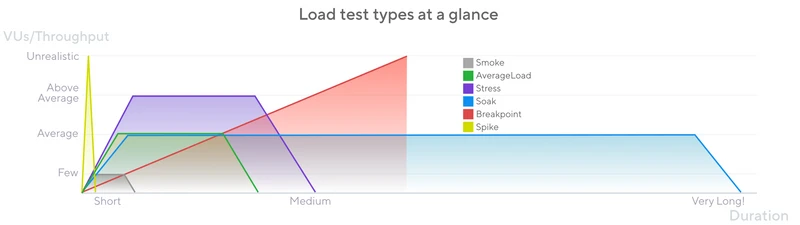
\includegraphics[width=1\textwidth]{./assets/figures/load-test-types.png}
  \caption{Types de tests de montée en charge~\cite{k6-load-test-types}.}
  \label{fig:load-test-types}
\end{figure}

\begin{itemize}
  \item \textbf{Smoke tests}: permettent de valider que le script de test fonctionne et que le système fonctionne correctement sous une charge minimale.
  \item \textbf{Average-load tests}: évaluent les performances du système dans des conditions normales prévues.
  \item \textbf{Stress tests}: évaluent les performances du système à ses limites, lorsque la charge dépasse la moyenne prévue.
  \item \textbf{Soak tests}: évaluent la fiabilité et les performances du système sur des périodes prolongées.
  \item  \textbf{Spike tests}: valident le comportement et la survie du système en cas d'augmentation soudaine, brève et massive de l'activité.
  \item \textbf{Breakpoint tests}: augmentent progressivement la charge afin d'identifier les limites de capacité du système.
\end{itemize}

Le type le plus utile dans l'état actuel de \gls{beeplace} est le \textbf{Breakpoint test}. En effet, ce type de test permet d'observer facilement si les optimisations réalisées sont efficaces. Plus la charge supportée avant que le système ne s'effondre est élevée, plus les optimisations sont utiles.

Dans le futur, afin de vérifier après les optimisations réalisées que le système supporte la charge nécessaire, des \textbf{Spike tests} et des \textbf{Stress tests} seront également réalisés. Ces tests permettent de vérifier que le système ne s'effondre pas sous une charge plus élevée que la moyenne prévue, dans le cas d'un afflux soudain de festivaliers par exemple.

\subsubsection{Architecture}

Le code est séparé en deux parties: le code générique permettant de rendre compatible k6 avec Socket.IO et le test en lui-même. Le code générique est placé dans un package nommé \mintinline[breaklines]{bash}{@beescreens/benchmarks} et est importé dans le test \mintinline[breaklines]{bash}{apps/beeplace/tests/load-tests}. Ce code pourrait, dans le futur, être utilisé pour tester d'autres applications du projet \gls{beescreens} implémentant également Socket.IO, comme Pimp My Wall par exemple.

\dirtree{%
  .1 /.
  .2 apps.
  .3 beeplace.
  .4 tests.
  .5 load-tests.
  .4 ....
  .3 ....
  .2 packages.
  .3 benchmarks.
  .3 ....
}

\subsubsection{Test avec K6}

Le test utilisé est une Breakpoint test, l'implémentation a été séparée en trois parties afin de pouvoir la commenter plus facilement.

\begin{listing}[H]
  \inputminted{ts}{assets/figures/breakpoint-test-1.ts}
  \caption{Breakpoint test avec k6 - Fonction principale}
  \label{listing:k6-breakpoint-test-1}
\end{listing}

La fonction principale de la figure \ref{listing:k6-breakpoint-test-1} est exécutée pour chaque utilisateur virtuel. Elle se connecte à l'endpoint WebSocket grâce à la classe \mintinline[breaklines]{ts}{K6SocketIo} du package précédemment évoqué \mintinline[breaklines]{bash}{@beescreens/benchmarks}. Elle appelle ensuite la fonction \mintinline[breaklines]{bash}{onConnect} détaillée dans la figure \ref{listing:k6-breakpoint-test-3} qui contient le comportement propre à l'utilisateur. Les erreurs sont également comptabilisées afin de les afficher à la fin du test.

\begin{listing}[H]
  \inputminted{ts}{assets/figures/breakpoint-test-2.ts}
  \caption{Breakpoint test avec k6 - Options}
  \label{listing:k6-breakpoint-test-2}
\end{listing}

La figure \ref{listing:k6-breakpoint-test-2} présente les options du test. Le test dure un maximum de 5 minutes et va ajouter un nombre d'utilisateurs virtuels croissant jusqu'à l'objectif souhaité de 1000 utilisateurs. Le test ne se soucie pas de l'éventuelle latence de l'application grâce à l'exécuteur \mintinline[breaklines]{bash}{ramping-arrival-rate}.

Le \mintinline[breaklines]{bash}{threshold} défini permet d'arrêter le test lorsque le temps de chargement est jugé trop conséquent pour une utilisation fluide de l'application. Dans cet exemple, le test s'arrête si le temps de connexion WebSocket dépasse 1200 millisecondes pour 95\% des utilisateurs virtuels.

\begin{listing}[H]
  \inputminted{ts}{assets/figures/breakpoint-test-3.ts}
  \caption{Breakpoint test avec k6 - Comportement des utilisateurs virtuels}
  \label{listing:k6-breakpoint-test-3}
\end{listing}

Finalement, la figure \ref{listing:k6-breakpoint-test-3} présente le comportement des utilisateurs virtuels. Chaque utilisateur virtuel se connecte à l'endpoint WebSocket et récupère le canvas actuel ainsi que les options de configuration. Il pose ensuite le nombre de pixels maximum (3 dans cet exemple) sur le canvas de manière aléatoire. Pour finir, il attend 10 secondes avant de se déconnecter afin de simuler la réception des pixels dessinés par les autres utilisateurs. Le nombre de pixels dessiné est comptabilisé afin de l'afficher dans les résultats du test.

\subsection{Résultats initiaux}

Les résultats des tests k6 contiennent de nombreuses métriques intéressantes. Les comparaisons vont se baser sur un échantillon d'entre elles mais un exemple complet est disponible au lien en note de bas de page \footnote{\url{https://github.com/heig-vkaelin/template-tb/blob/main/assets/external/k6-result.txt}}.

Les métriques utilisées pour pouvoir vérifier par la suite si les optimisations sont efficaces sont les suivantes:

\begin{itemize}
  \item Temps d'exécution du test avant que le seuil de latence ne soit atteint (1200 ms pour la connexion WebSocket).
  \item Nombre d'utilisateurs virtuels créés
  \item Nombre de pixels dessinés
\end{itemize}

Le test a été lancé 10 fois afin de prévenir les éventuelles erreurs de mesure. Les résultats sont présentés dans le tableau \ref{table:k6-initial-results}.

\begin{table}[H]
  \centering
  \begin{tabular}{|l|l|l|l|}
    \hline
    \textbf{Test}    & \textbf{Temps d'exécution} & \textbf{Utilisateurs virtuels} & \textbf{Pixels dessinés} \\ \hline
    1                & 22385.053 ms               & 703                            & 1317                     \\ \hline
    2                & 20921.705 ms               & 589                            & 1168                     \\ \hline
    3                & 22353.215 ms               & 704                            & 1366                     \\ \hline
    4                & 23175.281 ms               & 707                            & 1389                     \\ \hline
    5                & 30976.405 ms               & 797                            & 1672                     \\ \hline
    6                & 24097.739 ms               & 702                            & 1382                     \\ \hline
    7                & 25074.294 ms               & 699                            & 1319                     \\ \hline
    8                & 22141.945 ms               & 630                            & 1455                     \\ \hline
    9                & 32062.651 ms               & 786                            & 1596                     \\ \hline
    10               & 20743.08 ms                & 452                            & 1056                     \\ \hline
    \textbf{Moyenne} & \textbf{24393.147 ms}      & \textbf{676.9}                 & \textbf{1372}            \\ \hline
    \textbf{Médiane} & \textbf{22780.167 ms}      & \textbf{702.5}                 & \textbf{1374}            \\ \hline
  \end{tabular}
  \caption{Résultats initiaux des tests de montée en charge avec k6}
  \label{table:k6-initial-results}
\end{table}

La médiane sera préférée à la moyenne pour les futurs comparaisons car elle est moins sensible aux valeurs extrêmes. Même si les valeurs des 10 itérations du test sont relativement proches dans ce cas-ci.

Pour conclure, avec la version initiale de \gls{beeplace}, le test est exécuté pendant environ \textbf{23 secondes} en créant \textbf{702 utilisateurs virtuels} qui dessinent au total \textbf{1374 pixels}.

\section{Profiling}

Pour trouver plus facilement les optimisations à effectuer, il est nécessaire de profiler l'application. Le profiling permet de trouver les parties du code qui prennent le plus de temps à s'exécuter et qui sont donc plus intéressantes à optimiser.

\subsection{Choix de l'outil}

\subsubsection{Solution native à Node.js}

Node.js propose un outil de profiling natif qu'il est possible d'appeler en utilisant simplement l'argument \mintinline[breaklines]{bash}{node --prof}. Cet outil permet de générer un fichier de profiling illisible en lui-même. Heureusement, l'argument \mintinline[breaklines]{bash}{node --prof-process} permet d'analyser ce fichier de log et de générer un fichier textuel plus compréhensible.

L'inconvénient de cette approche est que le fichier texte des résultats reste pas très pratique à utiliser. Il est difficile de voir quelles fonctions sont les plus gourmandes en ressources sans une interface graphique.

\subsubsection{Parca}

Parca~\cite{parca} est un outil de profiling open-source développé par l'équipe derrière le projet Kubernetes. Son objectif est d'être très léger afin de pouvoir être utilisé en production sans affecter les performances de l'application. Ces performances sont possibles car Parca utilise une approche basée sur la technologie eBPF (extended Berkeley Packet Filter)~\cite{ebpf}. Cette technique permet d'exécuter du code dans le noyau Linux sans avoir besoin de modifier directement le code source.

Le problème de cette technique est qu'elle n'est pas supportée par tous les systèmes d'exploitation. Parca ne peut donc pas être utilisé sur Windows ou macOS. Il n'est donc pas possible de tester en local l'optimisation avec Parca dans le cadre du projet \gls{beeplace}. Cependant, Parca reste un choix intéressant lorsqu'il s'agira de tester l'optimisation sur le serveur de production.

\subsubsection{Pyroscope}

Pyroscope~\cite{pyroscope} est un outil de profiling également open-source développé par l'équipe Grafana Labs. Il s'agit de la même qui est derrière l'outil de tests de montée en charge k6 que \gls{beeplace} utilise. Pyroscope est utilise facilement en local avec Docker et propose une intégration avec de nombreux langages de programmation, dont Node.js. Il suffit d'ajouter la dépendance et de lancer le profiling dans le code de l'application. Le code enverra par la suite les données de profiling au serveur Pyroscope toutes les 10 secondes.

Malheureusement, le dashboard proposé n'est pas le plus intuitif, il ne met pas à disposition de nombreux filtres et cela rend l'analyse des résultats difficile.

\subsection{Clinic.js}

Clinic.js~\cite{clinicjs} est une suite d'outils de profiling développé par des membres de l'équipe derrière Node.js. Il suffit d'installer le projet comme une dépendance \gls{npm} globale pour avoir accès à 4 outils différents:

\begin{itemize}
  \item \textbf{Doctor} permet de diagnostiquer les problèmes de performance d'une applications en identifiant les symptômes tels que des problèmes de lecture/écriture ou des problèmes de mémoire.
  \item \textbf{Flame} permet d'identifier rapidement et précisément les goulots d'étranglement du code grâce à des graphiques en flammes qui visualisent les chemins d'exécution les plus fréquents.
  \item \textbf{Bubbleprof} observe les opérations asynchrones de l'application et les affiche dans un graphique en bulles pour visualiser les différents délais.
  \item \textbf{Heap Profiler} met également à disposition des graphiques en flammes comme le mode Flame mais pour l'utilisation de la mémoire.
\end{itemize}

Le mode le plus intéressant pour le projet \gls{beeplace} est le mode Flame. Il permet de visualiser les chemins d'exécution les plus fréquents et donc de trouver les fonctions qui prennent le plus de temps à s'exécuter. Celles-ci doivent donc être optimisées en priorité.

L'utilisation de Clinic.js est plus pensée pour le local. En effet, le rapport de profiling est généré lorsque l'application Node s'arrête. Ce qui n'est pas envisageable en production. Il est donc nécessaire de tester l'optimisation en local avant de la déployer sur le serveur de production.

\subsection{Solution choisie}

Le choix final s'est donc tourné vers un profiling en local à l'aide de Clinic.js afin d'avoir un retour rapide sur l'efficacité des optimisations réalisées. Pour récapituler, le processus est le suivant:

\begin{enumerate}
  \item Lancer l'application Node.js en local avec Clinic.js: \mintinline[breaklines]{bash}{clinic flame -- node app.js}
  \item Démarrer le test de montée en charge en local avec k6
  \item Arrêter l'application Node.js une fois le test terminé
  \item Analyser le rapport de Clinic.js
  \item Optimiser le code
  \item Recommencer
\end{enumerate}

Une fois les optimisations effectuées et testées en local, il est possible de les déployer sur le serveur de test de montée en charge pour comparer les résultats avec la version initiale \ref{table:k6-initial-results}.

\subsection{Analyses}

\subsubsection{Rapport initial}

% Used results: file:///Users/valentin/code/beescreens/apps/beeplace/backend/.clinic/59944.clinic-flame.html

\begin{figure}[H]
  \centering
  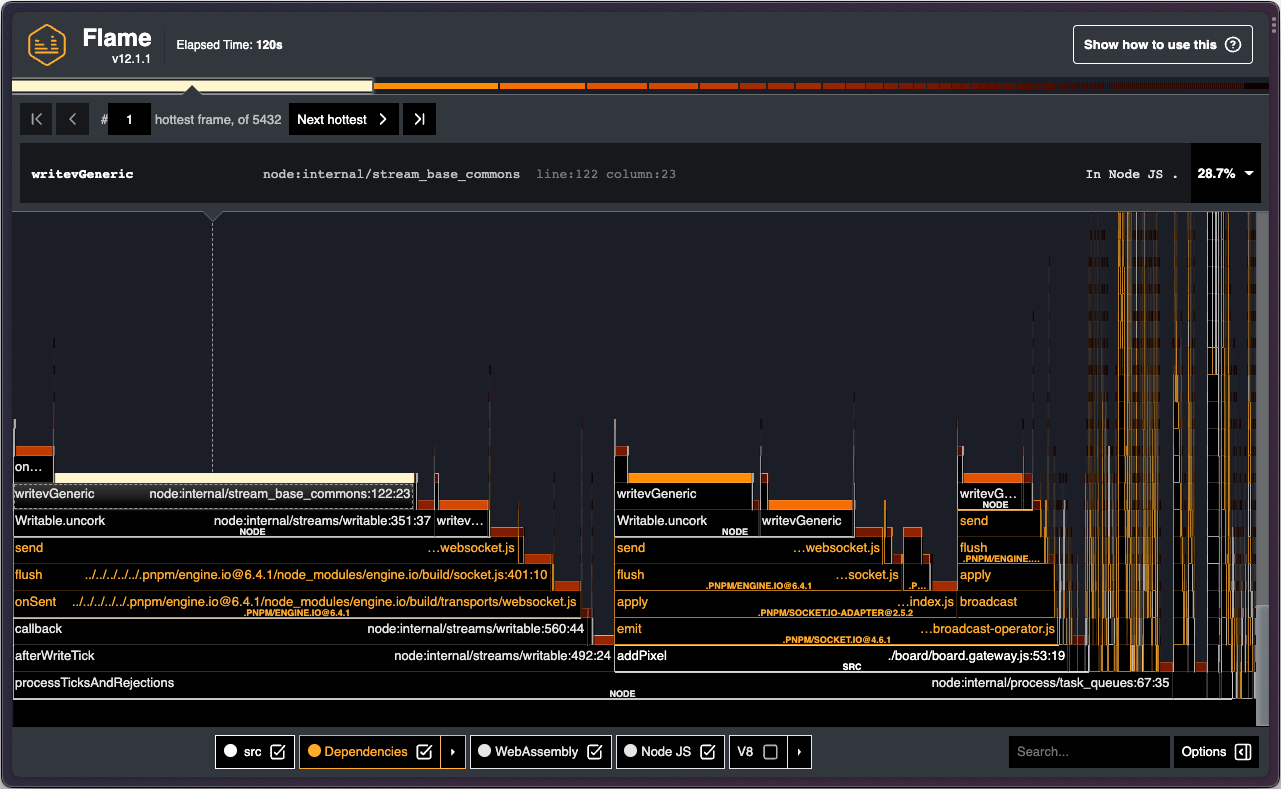
\includegraphics[width=1\textwidth]{./assets/figures/flame/flame1-overview.png}
  \caption{Vision d'ensemble du rapport initial de Clinic.js}
  \label{fig:flame1-overview}
\end{figure}

A la fin du test de montée en charge, l'analyse réalisée par Clinic.js avec son graphique en flammes visible sur la figure \ref{fig:flame1-overview} n'est pas facilement interpretable. En effet, initialement les fonctions ne sont pas filtrées. Le graphique affiche donc les fonctions venant du code Node.js ainsi que des dépendances en plus du code propre au projet. Il est tout de même possible de voir que la plupart des fonction affichées concernent l'écriture de données dans le cadre des WebSockets avec des fonctions comme \mintinline[breaklines]{javascript}{writevGeneric}, \mintinline[breaklines]{javascript}{onwrite} ou \mintinline[breaklines]{javascript}{flush}.

En filtrant pour garder uniquement le code du projet, car il s'agit du code qu'il est possible d'optimiser, le graphique devient plus lisible comme le montre la figure \ref{fig:flame1-filtered}.

\subsubsection{Rapport filtré}

\begin{figure}[H]
  \centering
  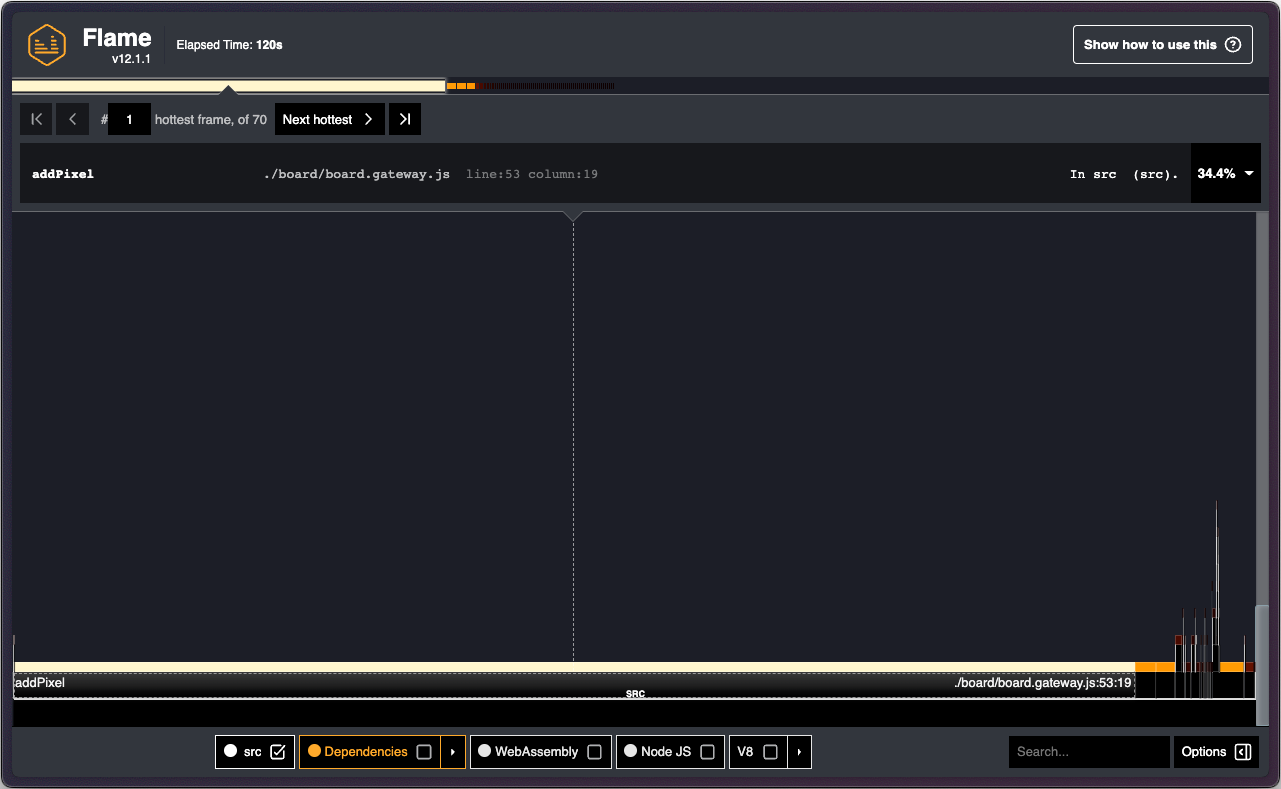
\includegraphics[width=1\textwidth]{./assets/figures/flame/flame1-filtered.png}
  \caption{Vision filtrée du rapport initial de Clinic.js}
  \label{fig:flame1-filtered}
\end{figure}

Plus de 34\% du temps d'exécution est passé dans la fonction \mintinline[breaklines]{javascript}{addPixel}. Celle-ci est appelée à chaque fois qu'un utilisateur envoie un nouveau pixel au serveur. Elle contient la logique suivante:

\begin{enumerate}
  \item Récupérer le nombre de pixels posés par l'utilisateur
  \item Ajouter le pixel dans le BitField Redis ainsi que dans l'historique PostgreSQL
  \item Incrémenter le nombre de pixels posés par l'utilisateur (ou le créer s'il n'existe pas)
  \item Partager le pixel avec les autres utilisateurs connectés (broadcast WebSockets)
\end{enumerate}

La deuxième fonction la plus utilisée est \mintinline[breaklines]{javascript}{placePixel} avec 0.7\% du temps d'exécution. Celle-ci s'occupe du point numéro 2. de la fonction \mintinline[breaklines]{javascript}{addPixel}. Elle est donc fortement liée à la fonction \mintinline[breaklines]{javascript}{addPixel}.

Les fonctions suivantes ne dépassent pas les 0.6\% du temps d'exécution, il s'agit notamment de la récupération de l'état actuel du BitField Redis ainsi que de l'initialisation de la connexion WebSockets.

Il faudra donc dans un premier temps se concentrer sur la fonction \mintinline[breaklines]{javascript}{addPixel}. Pour commencer, il est possible de regrouper les tâches de la fonction en deux catégories à optimiser:

\begin{enumerate}
  \item Sauvegarde du pixel
  \item Broadcast du pixel
\end{enumerate}

Afin de vérifier quelle partie doit être optimisée en priorité, il est possible de se concentrer sur la fonction \mintinline[breaklines]{javascript}{addPixel} et d'afficher à nouveau les fonctions des dépendances comme la figure \ref{fig:flame1-addPixel} le montre.

\subsubsection{Fonction addPixel}

\begin{figure}[H]
  \centering
  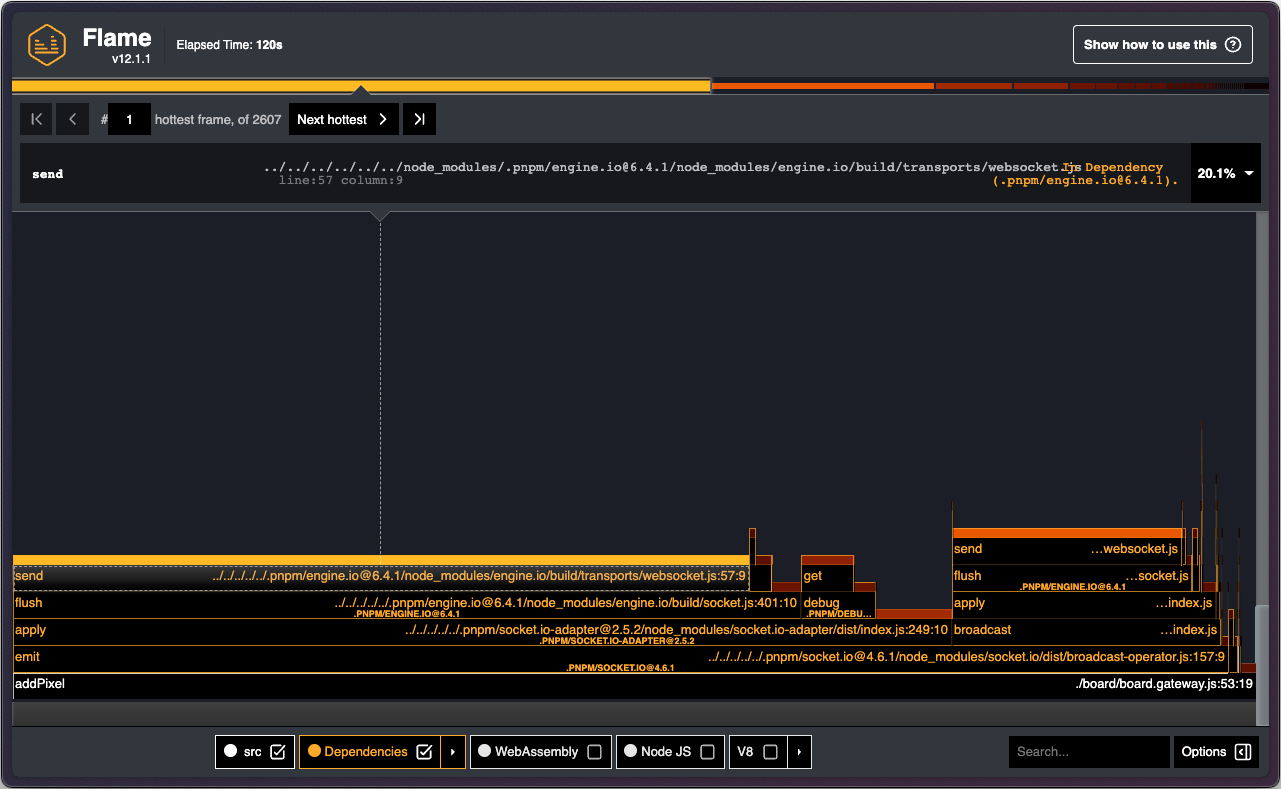
\includegraphics[width=1\textwidth]{./assets/figures/flame/flame1-addPixel.png}
  \caption{Zoom sur la fonction \mintinline[breaklines]{javascript}{addPixel} du rapport initial de Clinic.js}
  \label{fig:flame1-addPixel}
\end{figure}

Cette figure \ref{fig:flame1-addPixel} montre rapidement qu'une grande majorité du temps d'exécution de la fonction concerne le broadcast du pixel avec Socket.IO. En effet, la fonction \mintinline[breaklines]{javascript}{send} de Socket.IO représente 26.5\% du temps d'exécution de la fonction \mintinline[breaklines]{javascript}{addPixel} (20.1\% + 6.4\%). Concernant la sauvegarde du pixel, le temps d'exécution de la la fonction \mintinline[breaklines]{javascript}{placePixel} est si faible qu'il est affiché comme valant 0\% du temps d'exécution de la fonction \mintinline[breaklines]{javascript}{addPixel}.

\subsubsection{Conclusion initiale}

La fonction \mintinline[breaklines]{javascript}{addPixel} appelée à chaque fois qu'un utilisateur pose un pixel est clairement la fonction à optimiser en priorité. Plus précisément, la partie de la fonction qui s'occupe du broadcast le pixel avec Socket.IO à tous les autres utilisateurs connectés.

\section{Optimisations}
\label{sec:optimisations}

TODO